\documentclass{rapportAlgoM1}

\usepackage{mdframed}

%Définitions des auteurs
\newcommand{\auteurA}{Jean Dupont}
\newcommand{\auteurB}{Jean Dupond}
\newcommand{\auteurC}{}
\newcommand{\auteurD}{}

%Définition du sujet
\newcommand{\sujet}{Sujet n°1 : Calcul de $\pi$ par la méthode de Monte-Carlo}

%% Définitions pour le projet
\title{\LARGE{\titreGeneral}}%ne pas modifier
\author{\auteurA \\ \auteurB}% à modifier selon le nombre d'auteurs

\date{2022-23}

\begin{document}
\setlength{\parindent}{1cm}%ne pas modifier
%\setlength{\parskip}{1ex plus 0.5ex minus 0.2ex}

%%Page de garde rapport Master Info Algo et Complexité
%%RRaffin, 01/01/2023

\begin{titlepage}
%%Bordure
\AddToShipoutPicture*{%
	\setlength\unitlength{1mm}
	\put(0,0){\makebox(0,0)[lb]{\color{white}\rule{\paperwidth}{\paperheight}}}
	\put(0,0){\makebox(0,0)[lb]{\color{bleudefrance}\rule{25mm}{\paperheight}}}
	\put(15,190){\rotatebox{90}{%
		\makebox(0,0)[r]{\fontsize{30}{30}\color{orange!50!white}
		\bfseries \selectfont{Algorithmique et complexité M1}}}
	}
}

%%Logos

\includegraphics[height=2cm]{logos/logo-ub.png}
\hfill

\includegraphics[height=2cm]{logos/logo-ufr.png}

%%Université/UFR/IEM
\vspace{1cm} 
{\large{Université de Bourgogne, UFR Sciences et Techniques, Département I.E.M.}\par}

%%Titre
\vspace{2cm}
{\huge\bfseries Projet <<\ Algorithmique et complexité\ >>}\par

\vspace{2cm}
\mdfdefinestyle{mdframedStyle}{leftmargin=2cm,rightmargin=2cm,%
	innerleftmargin=0.5cm,innerrightmargin=1cm,%
	frametitlerule=true, frametitlebackgroundcolor=lightgray!50,userdefinedwidth=.8\textwidth,align=center}
\begin{mdframed}[style=mdframedStyle, frametitle={Groupe}]
\begin{large}
	\begin{itemize}
		\item [] \auteurA
		\item [] \auteurB
		\item [] \auteurC
	\end{itemize}
\end{large}
\end{mdframed}

\vspace{2cm}

%%Sujet

\begin{center}
\begin{tcolorbox}[text width=0.8\textwidth]
\large \sujet
\end{tcolorbox}
\end{center}


\vfill
{\hfill\large 2022-2023\par}

\end{titlepage}


%ne pas modifier

\tableofcontents
\newpage

%au besoin
%\listoffigures
%\listoftables

\section{Introduction}

Ce modèle est là pour vous fournir les outils de rédaction du rapport de projets M1 Algorithmique et Complexité. Il ne vous permettra pas d'apprendre la rédaction avec \LaTeX{} (il y a une section avec quelques liens pour cela : section~\ref{sec:doclatex}, p.~\pageref{sec:doclatex}).

Votre document doit inclure figures, schémas, algorithmes, éventuellement code de la manière la plus claire possible. Ce document doit vous y aider. Vous pouvez facilement taper du texte au kilomètre (\LaTeX{} fera la mise en page, inutile de modifier des espaces ou des pages), vous pouvez faire des références à des \texttt{label}, des pages, des sections et ne vous concentrer que sur le fond du texte.

C'est à vous ensuite d'avoir un discours rigoureux, justifié mathématiquement ou informatiquement, avec les bons exemples et les bonnes preuves de ce que vous avancez. N'oubliez pas la conclusion et les extensions possibles de vos travaux, cela montre aussi votre connaissance du domaine.

\section{Modules et fichiers}
Il est assez simple d'inclure des fichiers \TeX{} dans vos fichiers \TeX{}, et ainsi d'avoir une construction modulaire de votre document. Cela permet aussi d'activer ou non cette inclusion avant la compilation (en commentant avec \%) et d'accélerer la compilation ou de travailler sur un document partiel.

\vspace{1ex}

\hrule
Voilà le contenu du fichier inclus.

Cela reste du \LaTeX, donc maths $f(x)=x^12$, complexité $\varphi$ ou $O$, etc.

Une équation sans label :
$$
\begin{pmatrix}
	x&2\\
	f(x)&3
\end{pmatrix}
=\begin{matrix}
0&1\\
1&0\\
\end{matrix}
$$

Ou avec label : 
\begin{equation}
	\label{eq:aveclabel}
	\Delta(x) = \left\{
	\begin{aligned}
		&0 & \text{si\quad} &\frac{Z}{\varepsilon}=0\\
		&x^{23} & \text{\quad sinon}&\\
	\end{aligned}
	\right.
\end{equation}

Pour pouvoir y faire référence dans le texte : c'est l'équation~\ref{eq:aveclabel}, page~\pageref{eq:aveclabel} (notez le \~{}  espace insécable dans le source, pour éviter le retour à la ligne avant le numéro de l'équation).
\hrule
\vspace{1ex}


\section{Images}
Inclure une image, pour faire simple\footnote{D'autres options sont disponibles, comme proposer à \LaTeX{} un placement (sinon il s'arrange pour placer les images sur une imême page pour ne pas polluer le texte).} :
\begin{verbatim}
	\begin{figure}
		\includegraphics[width=0.3\textwidth]{fichier.png}
	\end{figure}
\end{verbatim}

\begin{figure}H
	\centering
	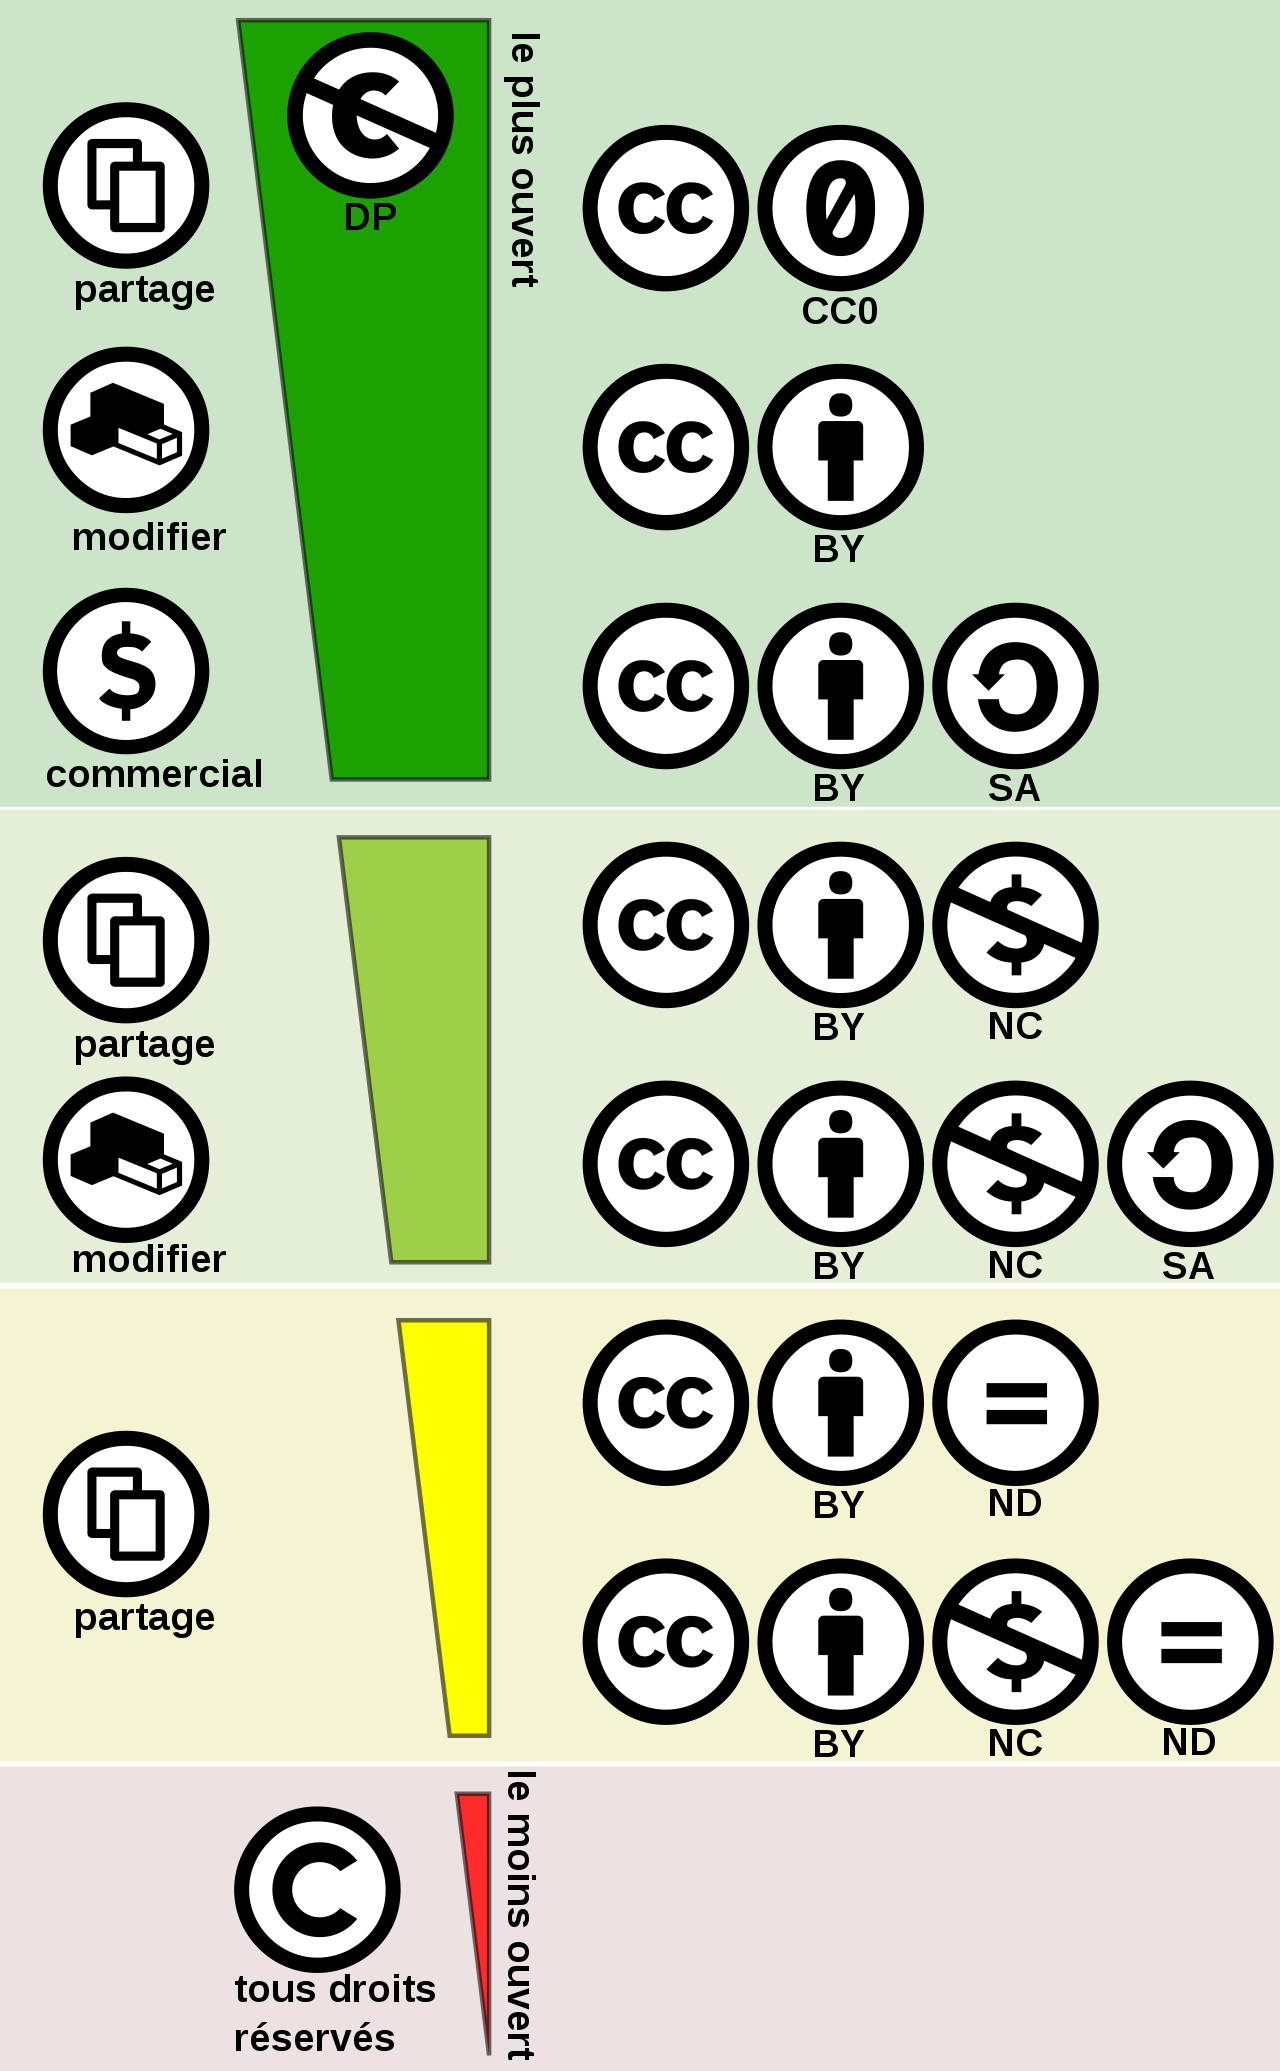
\includegraphics[width=0.3\textwidth]{images/creative_commons_license_spectrum_fr.png} %on utilise une taille relative au texte pour pouvoir s'adapter plus facilement
	\caption{Provient de \url{https://fr.wikipedia.org/wiki/Licence_Creative_Commons}}
	\label{fig:ccbysa}
\end{figure}

Comme l'image à un \verb+\label+, on peut y faire référence dans le texte (il le faut) pour l'expliquer. On a donc ici (page~\pageref{fig:ccbysa}) la figure~\ref{fig:ccbysa} qui donne les modes de licences Creative Commons, car c'est aussi important de vérifier que les images, documents inclus sont libres de droits.

L'environnement \verb+subfigure+ permet de grouper plusieurs figures, d'y ajouter des index et de faire référence à chacune. Du coup, on peut référencer la figure de gauche~\ref{fig:subfig1} ou celle de droite~\ref{fig:subfig2}, ou bien la figure complète~\ref{fig:subfigureComplete}.

\begin{figure}
	\centering
	\begin{subfigure}[b]{0.3\textwidth}
		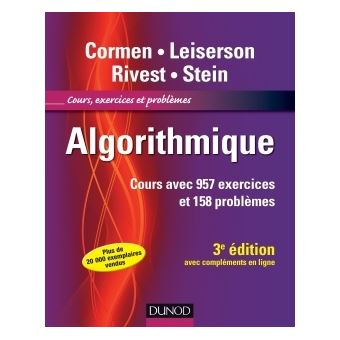
\includegraphics[width=\textwidth]{images/livreAlgoRivest.jpg}
		\caption{$y=f(x)$}
		\label{fig:subfig1}
	\end{subfigure}
	\quad
	\begin{subfigure}[b]{0.3\textwidth}
		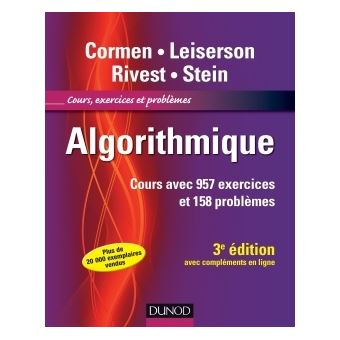
\includegraphics[width=\textwidth]{images/livreAlgoRivest.jpg}
		\caption{ou du texte}
		\label{fig:subfig2}
	\end{subfigure}
	\caption{Titre général de la figure}
	\label{fig:subfigureComplete}
\end{figure}


\section{Code}
On peut inclure facilement du code, à partir du fichier source (cela permet une mise à jour facile). Cela évite aussi d'utiliser l'environnement \verb+verbatim+ qui n'est pas adapté aux langages informatique. Comme d'habitude, on peut y mettre un \verb+label+ et l'utiliser. Ici le code source est le listing~\ref{code:caml}.

\lstinputlisting[inputpath=sources/, caption=Un programme OCaml (\lstname), label=code:caml]{fractionEgyptienne.caml}

\section{Références}
Si on doit citer des documents, des sites web, on utilise une bibliographie. Deux façons sont possibles, des \verb+bibitem+ qu'il faut écrire de la même façon (titre, auteur, année...) ou l'utilisation de \verb+bibtex+ qui fait le travail de gestion pour vous. J'ai choisi la seconde, c'est un peu plus long (il faut compiler le fichier .tex, puis le .bib, puis le .tex à nouveau), mais cela permet de copier-coller facilement des fichier \textit{bibtex} disponibles un peu partout.

Par exemple, j'ai copié les références du livre de Cormen et al depuis cette  \href{https://www.bibsonomy.org/bibtex/2225d42638921bee01b4ac8ff991b0a6a/rekstorm}{url} (trouvée par un moteur de recherche), j'ai collé le code\textit{ bibtex} dans le fichier \verb+references.bib+. Et voilà !

Je peux donc citer le livre~\cite{CormenIntroductionAlgo} facilement, et même avoir des styles de citations différents (alphabétiques, numériques), sans m'en occuper (ici le style imposé est \verb+apalike+). Si vous utilisez Overleaf (en ligne) ou TexStudio (en local), les phases de compilation sont automatiques à la génération du fichier PDF résultat, et les citations sont aidées par le logiciel (connaît les entrées du fichier .bib). De plus, seuls les références citées seront listées à la fin de ce rapport, pas d'oubli possible.

Je peux également citer les papiers de Dijkstra~\cite{Dijkstra1959} ou de Knuth~\cite{Knuth1997} qui sont fondateurs.

\section{Commandes}
Vous pouvez définir des commandes, si vous désesperez de taper Dikjstra, Dijstra ou Dijkstra en vous trompant.

\begin{verbatim}
	\newcommand{\dij}{Dijkstra}
\end{verbatim}
\newcommand{\dij}{Dijkstra} %se place plutôt avant le begin document pour en profiter partout
et voilà : \dij.

\section{Conclusion}
Ce document est un peu court, j'espère qu'il est suffisant pour démarrer votre rapport sans vous prendre la tête. Si vous avez des modifications à faire, n'hésitez pas à me les soumettre par \href{mailto:romain.raffin@u-bourgogne.fr}{mail}. Il y a moult choses à faire avec \LaTeX{}, qui peuvent réellement vous faciliter l'écriture de rapports, mémoires, thèses. Ce langage est un peu ardu les premiers temps mais la facilité de composition et la concentration de la rédaction sur le fond plutôt que la forme sont de vrais atouts.

%%annexes
\section*{Annexes}
\subsection{Docs Latex}\label{sec:doclatex}
\begin{itemize}
	\item \url{https://fr.wikibooks.org/wiki/LaTeX}
	\item \url{https://www.overleaf.com/learn}
	\item \url{https://www.learnlatex.org/fr/}·
	\item \url{https://latex-tutorial.com}
\end{itemize}

%%bibliographie
%utile seulement si le language est [french, english] \selectlanguage{french}
\bibliographystyle{apalike} % style des références
\bibliography{references} %fichier references.bib


\end{document}
